\documentclass{beamer}
\usepackage[dutch]{babel}
\usepackage{graphicx}
\usepackage{siunitx}
\usepackage{underscore}

\title{Project Microcontrollers}
\subtitle{Spacegame op POV-Display}
\author{Marieke Louage \and Stef Pletinck}
\institute{UGent Campus Kortrijk}
\date{17 mei 2019}
\logo{
\includegraphics[height=2cm]{img/logo.png}}

\begin{document}

\frame{\titlepage}

\begin{frame}
  \frametitle{Inhoud}
  \tableofcontents
\end{frame}

\section{Idee}
\begin{frame}
  \frametitle{Het Idee}
  \begin{itemize}
  \item<1-> Multiplayer spel
  \item<2-> Rond scherm (hardeschijfklok)
  \item<3-> Space Shooter
  \end{itemize}
\end{frame}

\section{Structuur}
\begin{frame}
  \frametitle{Structuur}
  \begin{center}
    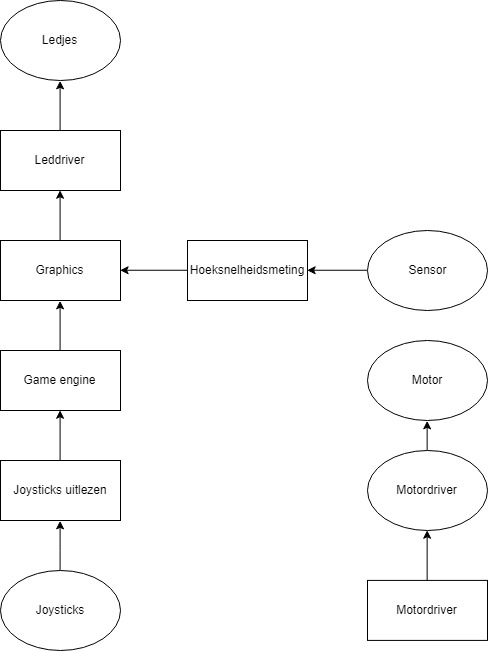
\includegraphics[height=0.8\textheight]{img/structuur.jpg}
  \end{center}
\end{frame}

\section{Werking Display}
\begin{frame}
  \frametitle{Werking Display}

  \begin{columns}
    \column{0.5\textwidth}
    \begin{itemize}
    \item Schijf verdeeld in verlichte sectoren
    \item Schijf met gaatjes in spiraal
    \item Optische sensor
    \item Snelle DC-Motor
    \end{itemize}

    \column{0.5\textwidth}
    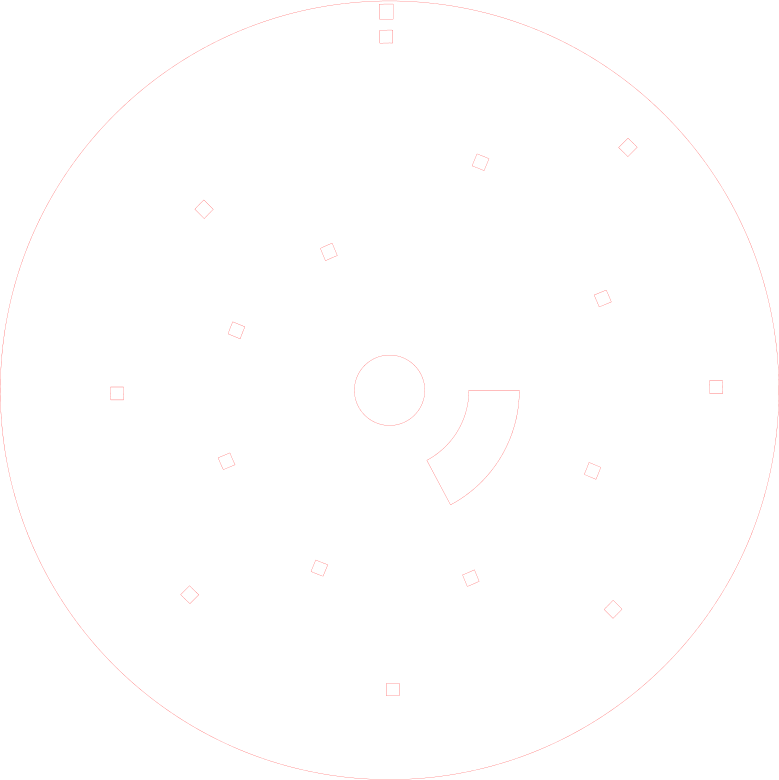
\includegraphics[width=0.9\textwidth]{img/schijf.jpg}
  \end{columns}
\end{frame}

\section{Motordriver}
\begin{frame}
  \frametitle{Motordriver}

  Een softwaredriver stuurt een ESC\footnote{Electronic Speed Control} module
  aan, die de eigenlijke brushless DC-motor aanstuurt. blabla blablablaa blalbalblaa
\end{frame}

\section{LEDs}
\begin{frame}
  \frametitle{LEDs}

  \begin{columns}
    \column{0.5\textwidth}
    \begin{itemize}
    \item \texttt{APA102} ledstrip
    \item 32 bits per LED
    \item Start- en endframe
    \item SPI
    \end{itemize}

    \column{0.5\textwidth}
    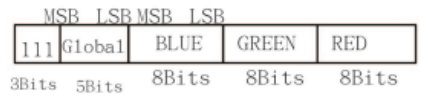
\includegraphics[width=0.9\textwidth]{img/ledpakket.png}
  \end{columns}
\end{frame}

\begin{frame}
  \frametitle{LEDs}
  \framesubtitle{SPI}

  \begin{itemize}
  \item 2 Mogelijkheden: Blocking en interruptgebaseerd
  \item 2 Klokcycli per bit
  \item \SI{68}{\micro\second} hele strip
  \end{itemize}
\end{frame}

\section{Graphics}
\begin{frame}
  \frametitle{Graphics}
\end{frame}

\section{Hoeksnelheidsmeting}
\begin{frame}
  \frametitle{Hoeksnelheidsmeting}
\end{frame}

\section{Game Engine}
\begin{frame}
  \frametitle{Game Engine}

  30 keer per seconde is er een \emph{tick}, ondertussen gebeuren er continu \emph{renders}.
  Er is ook enige debugfunctionaliteit.
\end{frame}

\begin{frame}
  \frametitle{Game Engine}
  \framesubtitle{De Tick}

  \begin{block}{Timing}
    \begin{itemize}
    \item 8-bits Timer/Counter in CTC
    \item \SI{30}{\hertz}
    \item \texttt{maybe_tick()}
    \end{itemize}
  \end{block}

  \begin{block}{Taken}
    \begin{itemize}
    \item Start- en eindscherm
    \item Input
    \item Updates
    \item Botsingen
    \item Test voor einde spel
    \end{itemize}
  \end{block}
\end{frame}

\begin{frame}
  \frametitle{Game Engine}
  \framesubtitle{Render}

  \begin{itemize}
  \item Continu
  \item Aanmaken Sprites
  \item Aansturen \emph{graphics}
  \end{itemize}
\end{frame}

\section{Joysticks}
\begin{frame}
  \frametitle{Joysticks}

  \begin{block}{Fysiek}
    \begin{itemize}
    \item 8 Microswitches
    \item Pullups
    \end{itemize}
  \end{block}

  \begin{block}{Software}
    \begin{itemize}
    \item Uitlezen pins
    \item \texttt{JoyStatus}
    \item Stijgende flanken
    \item Gemaksfuncties
    \end{itemize}
  \end{block}
\end{frame}

\section{Fysieke constructie}
\begin{frame}
  \frametitle{Fysieke constructie}

  \begin{block}{Schijf}
    De draaischijf bestaat uit \SI{3}{\milli\metre} dikke, zwarte ABS,
    uitgesneden op een lasercutter.
  \end{block}

  \begin{block}{Behuizing}
    De behuizing is gelasercut uit MDF, met een plexiglas afdekscherm.
  \end{block}

  \begin{block}{Achterplaat}
    Achter de draaischijf zit een achtergrond van met de hand uitgesneden, witte
    plasticfolie. Deze folie zorgt ook voor schermen tussen de sectoren.
  \end{block}
\end{frame}

\section{Mogelijke verbeteringen}
\begin{frame}
  \frametitle{Mogelijke Verbeteringen}
  
\end{frame}

\section{Conclusie}
\begin{frame}
  \frametitle{Conclusie}
  
\end{frame}

\end{document}